\documentclass[a4paper,11pt,UTF8]{article}
\usepackage{ctex}
\usepackage{amsmath,amsthm,amssymb,amsfonts}
\usepackage{amsmath}
\usepackage[a4paper]{geometry}
\usepackage{graphicx}
\usepackage{microtype}
\usepackage{siunitx}
\usepackage{booktabs}
\usepackage[colorlinks=false, pdfborder={0 0 0}]{hyperref}
\usepackage{cleveref}
\usepackage{esint} 
\usepackage{graphicx}
\usepackage{ragged2e}
\usepackage{pifont}
\usepackage{extarrows}
\usepackage{mathptmx}
\usepackage{float}
\usepackage{caption}
\captionsetup[figure]{name={Figure}}

\title{Microelectronics Circuit Analysis and Design Homework(11st)}
\author{Yuejin Xie \quad U202210333}
\date{Oct 23rd, 2023}
\begin{document}
\maketitle
10.44 Consider the MOSFET current-source circuit in Figure P10.44 with $V^+=+ 2.5$V and $R= 15$ k$\Omega$. The transistor parameters are $V_{TN}= 0.5$V$, k_n^{\prime}= 80\mu\mathrm{A/V}^{2},W/L=80\mu$A$/V^2, W/L= 6$, and $\lambda=0$. Determine $I_{\mathrm{REF}},I_{O}$, and $V_{DS2}( $sat$) .$
\begin{figure}[H]
	\centering
	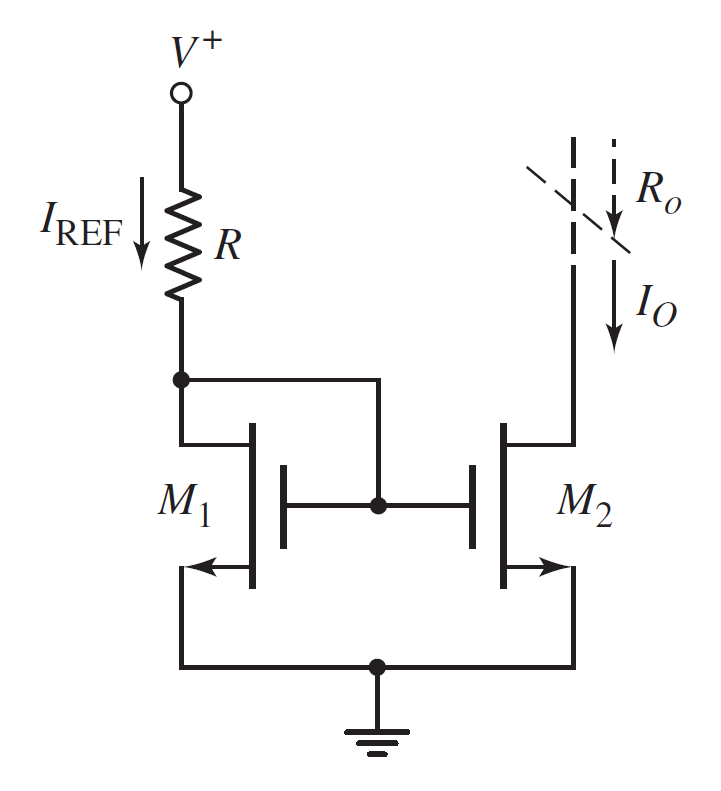
\includegraphics[width=0.4\textwidth]{10.44}
	\caption{Problem 10.44}
\end{figure}
10.54 The transistor circuit shown in Figure P10.54 is biased at $V^+=+5$V and $V^{-}=-5$ V.The transistor parameters are $V_{TP}=-1.2 V, k_p^{\prime}=80\mu A/N^2,\lambda=0,(W/L)_1=(W/L)_2=25,\mathrm{~and~}(W/L)_3=(W/L)_4=4.$ 
Determine $I_\mathrm{REF},I_O$, and $V_{SD2}$(sat).
\begin{figure}[H]
	\centering
	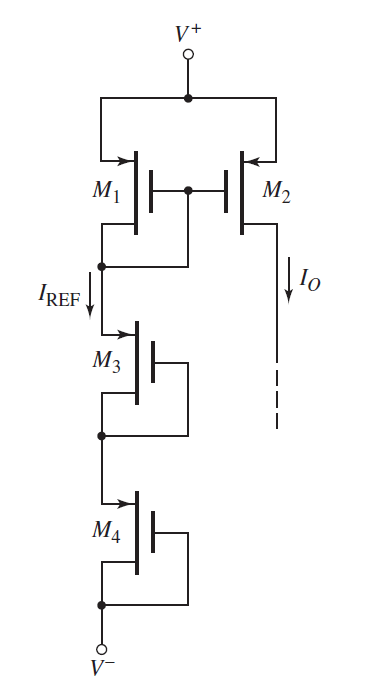
\includegraphics[width=0.4\textwidth]{10.54}
	\caption{Problem 10.54}
\end{figure}
10.60 The transistors in the circuit shown in Figure P10.60 have parameters $V_{TN}= 0.4$V$, V_TP= - 0.4$V$, k_n^{\prime}= 100\mu$A$/N^2, k_{p}^{\prime}= 60\mu$A$/\mathrm{V} ^2, $and $\lambda_n=\:\lambda_p=0.$ The transistor width-to-length ratios are $(W/L)_1=$ e $I_{O}, I_{\mathrm{REF}}, $and $(W/L)_{2}=20,\:(W/L)_{3}=5$, and $(W/L)_{4}=10$. Determine $V_{DS2}( $sat$) .$ What are the values of$V_GS1, V_{GS3}$, and $V_{SG4}?$
\begin{figure}[H]
	\centering
	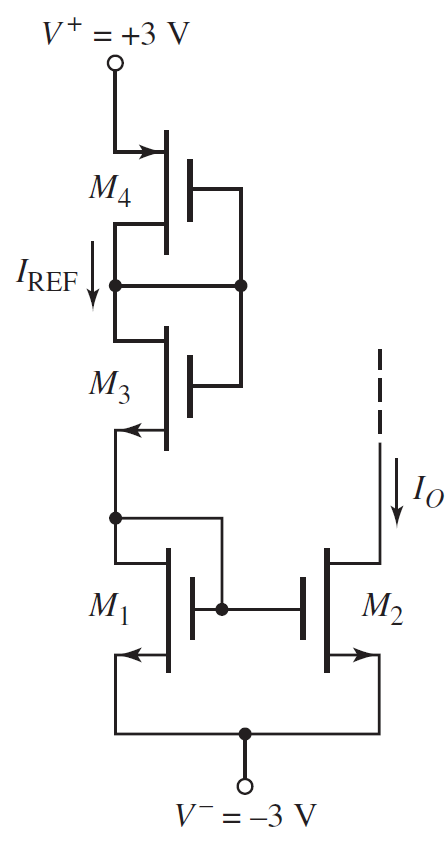
\includegraphics[width=0.4\textwidth]{10.60}
	\caption{Problem 10.60}
\end{figure}
10.84 In the circuit in Figure P10.84, the active load circuit is replaced by Wilson current source. Assume that $\beta=80$ for all transistors, and that $= 0.2$mA. Determine the open-circuit small-signal voltage gain.
\begin{figure}[H]
	\centering
	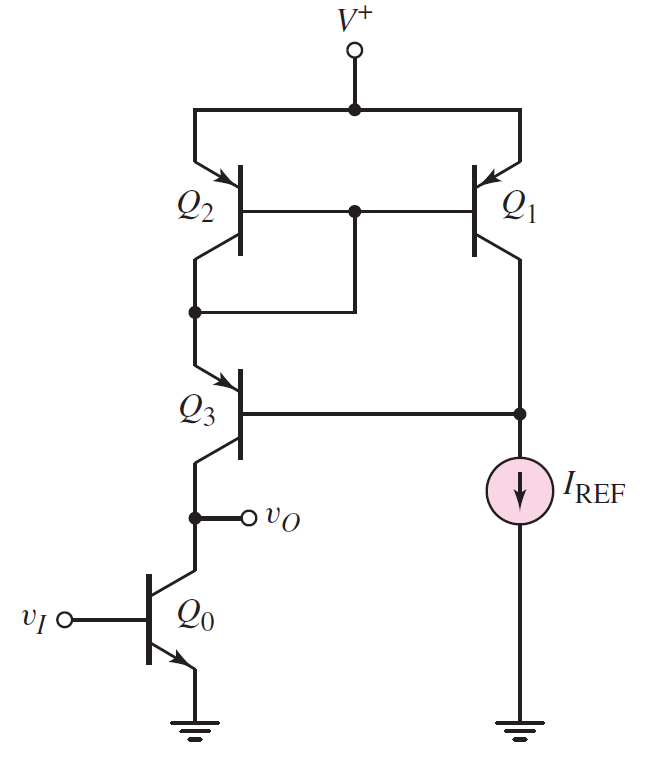
\includegraphics[width=0.4\textwidth]{10.84}
	\caption{Problem 10.84}
\end{figure}	
\end{document}